\documentclass[a4paper]{article}

\usepackage[pdftex]{graphicx}
\usepackage[margin=3cm]{geometry}
\usepackage{verbatim,moreverb,amssymb,amsmath}


\newcounter{question}
\newcommand{\question}[1]{\refstepcounter{question}\section*{Question~\thequestion~~~\small\emph{(#1)}}}
\renewcommand*\thequestion{\arabic{question}}


\begin{document}

\pagestyle{empty}
\thispagestyle{empty}



\noindent
\begin{minipage}{\columnwidth}
  \centering
  \Large
  DA4002 (HT11) Halmstad University\\
  Introduction to Algorithms, Data Structures, and Problem Solving\\[3\baselineskip]
  \Huge
  Written Exam\\
  \Large
  Thursday, January 10, 2013\\[2\baselineskip]
  Examiner: Roland Philippsen
\end{minipage}

\vfill

\noindent
\begin{center}
\fbox{
  \begin{minipage}{0.8\columnwidth}
    \textbf{Student Name:}\\[3\baselineskip]
  \end{minipage}
}
\end{center}

\vfill



\section*{Rules}

Aside from the obvious rules of conduct exams (e.g.\ no chatting):

\begin{itemize}
\item
  \textbf{No computing devices} (laptops, phones, calculators, \emph{etc}).
\item
  \textbf{No books or printouts} except for non-electronic dictionaries.
\item
  \textbf{Allowed hand-written notes}: two sheets of A4 paper (front and back).
\end{itemize}



\section*{General Guidelines}

\begin{itemize}
\item
  \textbf{Read carefully} and pace yourself.
  You can solve the problems in any order you want, but later problems may be easier to solve after you have answered the preceding questions.
\item
  \textbf{Write clearly} and draw clear diagrams.
  If you need to correct a mistake, then cleanly cross out the wrong answer and clearly indicate where the correction can be found.
\item
  \textbf{Indicate the question number} for each of your answers.
  If a question has sub-questions, indicate the sub-question number after the main question number, separated by a dot.
  For example, question 3 has 4 sub-questions, and their answers should be numbered 3.1, 3.2, 3.3, and 3.4.
\end{itemize}



\pagebreak
\pagestyle{plain}
\thispagestyle{plain}
\setcounter{page}{1}



\question{5 points}

% 0.5 pts each for the lists
% 1 pt each for the trees and graphs

Below are six diagrams labelled \textbf{(A)}, \textbf{(B)}, \textbf{(C)}, \textbf{(D)}, \textbf{(E)}, and \textbf{(F)}.
Each of them shows a data structure containing items of value $\{1, 2, 3, 4, 5, 6, 7\}$.

\vfill

\begin{center}
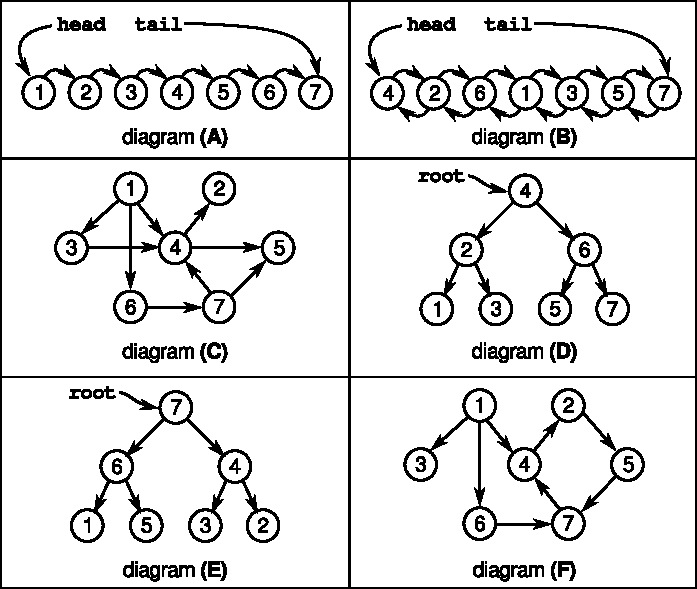
\includegraphics[width=0.8\columnwidth]{ds.pdf}
\end{center}

\vfill

\noindent
Match each data structure diagram with one of the data structure names in the table below.
Use the most specific data structure name for each diagram.

\vfill

\begin{center}
  \begin{tabular}{|p{0.3\columnwidth}|p{0.3\columnwidth}|}
    \hline
    data structure name & diagram label \\
    \hline
    & \\
    \textbf{singly linked list} & \\
    & \\
    \hline
    & \\
    \textbf{doubly linked list} & \\
    & \\
    \hline
    & \\
    \textbf{binary search tree} & \\
    & \\
    \hline
    & \\
    \textbf{max heap} & \\
    & \\
    \hline
    & \\
    \textbf{directed graph} & \\
    & \\
    \hline
    & \\
    \textbf{directed acyclic graph} & \\
    & \\
    \hline
  \end{tabular}
\end{center}


\clearpage


\question{5 points}

% 0.5 pts for each calculation

Answer the following questions about computational complexity.
\emph{\textbf{Notice the table of numeric values} for $x^2$ and $2^x$ on the bottom of this page, to help you with the computations.}


\begin{enumerate}
  
\item
  Algorithm \textbf{A} has exponential complexity: $T_A\in O(2^N)$.
  Its running time for a problem of size $N=256$ has been measured to be $T_A=100ms$.
  
  How much time $T_A'$ will this algorithm require to solve a problem of size $N'=260$?

\item
  Each of the five algorithms \textbf{B}, \textbf{C}, \textbf{D}, \textbf{E}, and \textbf{F} also took $T_i=100ms$ to solve a problem of size $N=256$.
  Fill in the following table with the time $T_i'$ that each of these algorithms requires to solve a problem of size $N'=1024$.
  Note that the table gives a different complexity class for each algorithm.
  
  \begin{tabular}{|p{0.2\columnwidth}l|p{0.4\columnwidth}|}
    \hline
    \emph{complexity} && \emph{time} $T_i'$ \\
    \hline
    && \\
    $T_B\in O(N^2)$ & quadratic & \\
    && \\
    \hline
    && \\
    $T_C\in O(N)$ & linear & \\
    && \\
    \hline
    && \\
    $T_D\in O(N\log N)$ && \\
    && \\
    \hline
    && \\
    $T_E\in O(\log N)$ & logarithmic & \\
    && \\
    \hline
    && \\
    $T_F\in O(1)$ & constant & \\
    && \\
    \hline
  \end{tabular}
  
\item
  A logarithmic algortihm \textbf{G} took $T_G=1s$ on a problem of size $N=8$.
  How big of a problem can it solve if the available time is $4s$?
  
\item
  Each of the three following algorithms \textbf{H}, \textbf{I}, and \textbf{J} also took $T_i=1s$, but on problems of size $N=1024$.
  Fill in the following table with the problem sizes $N'$ that can be solved when there are $4s$ available.
  Again, the table gives a different complexity for each algorithm.
  
  \begin{tabular}{|p{0.2\columnwidth}l|p{0.4\columnwidth}|}
    \hline
    \emph{complexity} && \emph{problem size} $N'$ \\
    \hline
    && \\
    $T_H\in O(2^N)$ & exponential & \\
    && \\
    \hline
    && \\
    $T_I\in O(N^2)$ & quadratic & \\
    && \\
    \hline
    && \\
    $T_J\in O(N)$ & linear & \\
    && \\
    \hline
  \end{tabular}

\end{enumerate}

\vfill

\small

\noindent
\begin{tabular}{|l|r|r|r|r|r|r|r|r|r|r|r|r|r|}
  \hline
  $x=$   & 0 & 1 & 2 &  3 &  4 &   5 &   6 &   7 &   8 &   9 &   10 &   11 &   12 \\
  \hline
  $x^2=$ & 0 & 1 & 4 &  9 & 16 &  25 &  36 &  49 &  64 &  81 &  100 &  121 &  144 \\
  $2^x=$ & 1 & 2 & 4 &  8 & 16 &  32 &  64 & 128 & 256 & 512 & 1024 & 2048 & 4096 \\
  \hline
\end{tabular}

\hfill
\begin{tabular}{|l|r|r|r|r|r|r|r|r|}
  \hline
  $x=$   &   13 &    14 &    15 &    16 &     17 &     18 &     19 &      20 \\
  \hline
  $x^2=$ &  169 &   196 &   225 &   256 &    289 &    324 &    361 &     400 \\
  $2^x=$ & 8192 & 16384 & 32768 & 65536 & 131072 & 262144 & 524288 & 1048576 \\
  \hline
\end{tabular}
\normalsize

\clearpage


\question{6 points}

% 1 pt for each sub-question (although the first two are insultingly simple)

The runtime of two programs \textbf{X} and \textbf{Y} has been measured in microseconds ($1\mu s=10^{-6}s$) for various problem sizes $N$.
Also, the measured time has also been divided by $N^2$ and $N\log N$, as shown in the table below:
on the left are the plots for program \textbf{X},
and the right shows the plots for program \textbf{Y}.

\begin{center}
  \begin{tabular}{|l|c|c|}
    \hline
    &
    \textbf{Program X} &
    \textbf{Program Y} \\
    \hline
    \textbf{Time} &
    $T_X(N)$ &
    $T_Y(N)$ \\
    &
    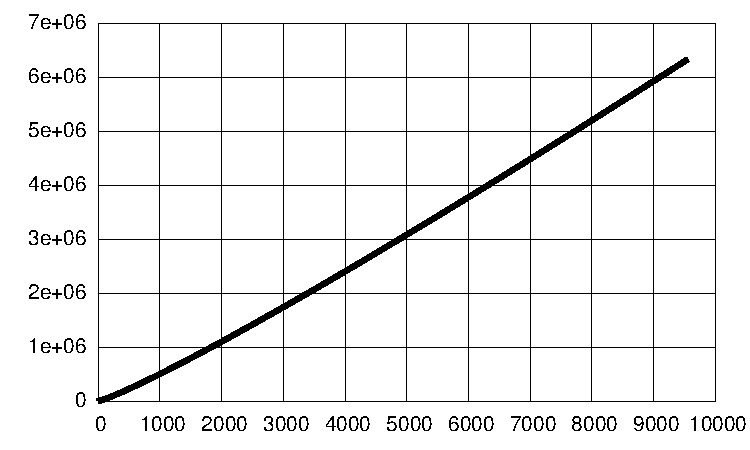
\includegraphics[width=0.44\columnwidth]{onln.pdf} &
    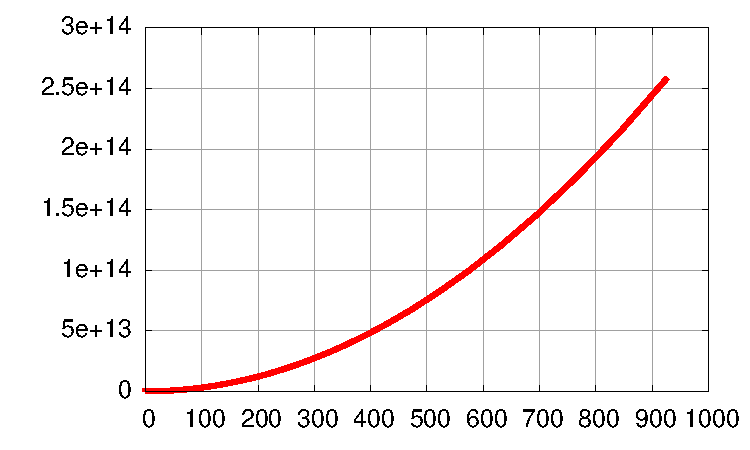
\includegraphics[width=0.44\columnwidth]{on2.pdf} \\
    \hline
    $O(N^2)$ &
    $T_X/N^2$ &
    $T_Y/N^2$ \\
    &
    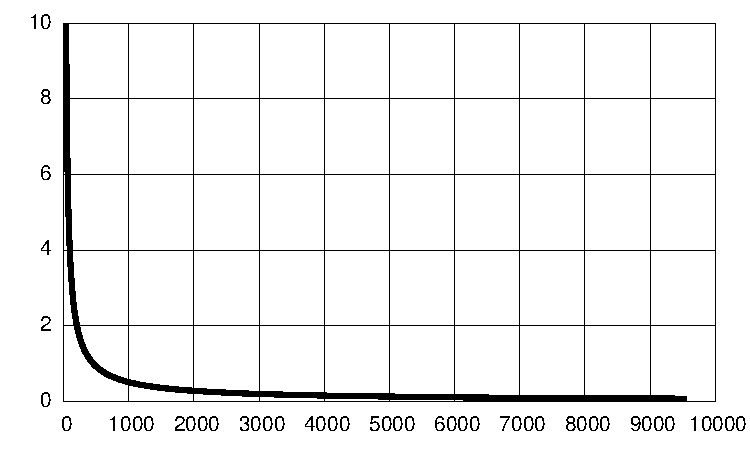
\includegraphics[width=0.44\columnwidth]{onln_n2.pdf} &
    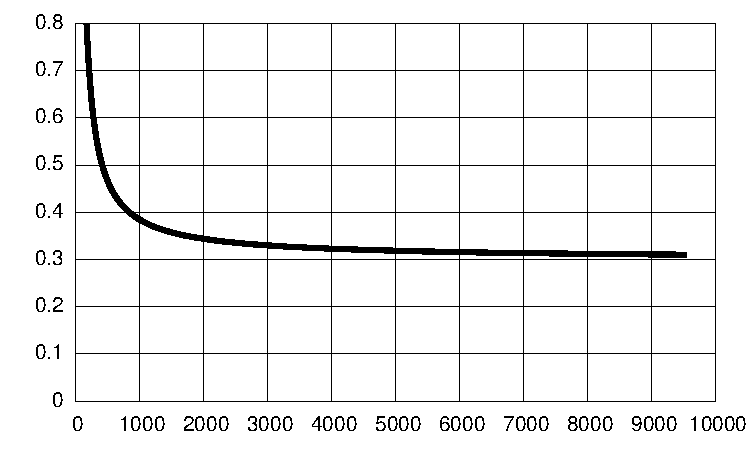
\includegraphics[width=0.44\columnwidth]{on2_n2.pdf} \\
    \hline
    $O(N\log N)$ &
    $T_X/(N\log N)$ &
    $T_Y/(N\log N)$ \\
    &
    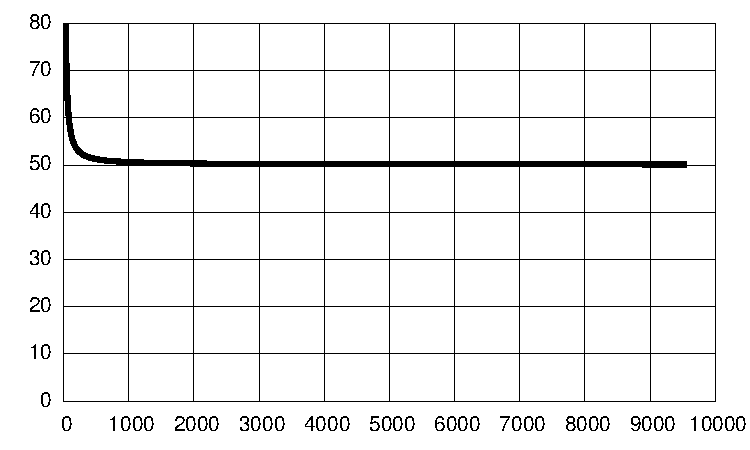
\includegraphics[width=0.44\columnwidth]{onln_nln.pdf} &
    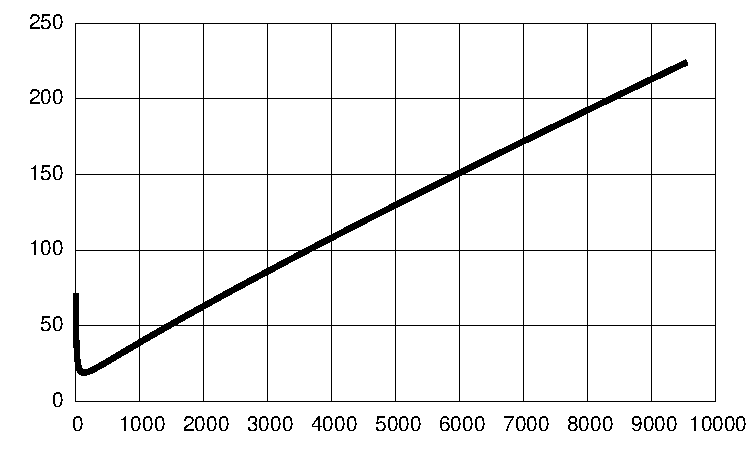
\includegraphics[width=0.44\columnwidth]{on2_nln.pdf} \\
    \hline
  \end{tabular}
\end{center}

\vfill

\noindent
Answer the following questions.
\emph{\textbf{Notice the table of numeric values} for $x^2$ and $2^x$ on the bottom of the previous page, to help you with sub-questions 5 and 6.}

\begin{enumerate}
\item
  How big of a problem (approximately) can program \textbf{X} solve in $T=2s=2\cdot10^6 \mu s$?
\item
  How big of a problem (approximately) can program \textbf{Y} solve in $T=20s=2\cdot10^7\mu s$?
\item
  What is the complexity class of program \textbf{X}?
\item
  What is the complexity class of program \textbf{Y}?
\item
  How long will program \textbf{X} run (approximately) for a problem of size $N=10^6$?
\item
  How long will program \textbf{Y} run (approximately) for a problem of size $N=2\cdot 10^5$?
\end{enumerate}


\clearpage

\question{9 points}

% 3 pts for the backtrace (3 solution paths that all yield the same end result)
% 6 pts for the second table (1 pt per correct row, but be nice concerning ``Folgefehler'')

Dynamic programming can be used to choose coins that add up to a given amount, such that the number of coins is minimal.
The following table shows this when the available coins are $C=\{1, 4\}$, for total amounts of up to $K=6$.

The \emph{value} $F(K)$ stands for the minimum amount of coins to create a total of $K$.
At each step, it is the minimum of the available options $f_1(K)$ and $f_4(K)$.
Thus, $F$ is computed using $F(K)=\min(f_1(K), f_4(K))$.
If an option is not available for a given step, it is marked $\varnothing$.
Notice hat the table starts at $K=0$, where $F(0)=0$.

\begin{center}
  \begin{tabular}{|c|l|l|l|c|}
    \hline
    \textbf{step} &
    \multicolumn{3}{|c|}{\textbf{choices}} &
    \textbf{value}
    \\
    $K$ &
    cost of $c=1$ &
    cost of $c=4$ &
    \textbf{best} $c$ &
    $F$ \\
    \hline
    $0$ &
    $\varnothing$ &
    $\varnothing$ &
    $\varnothing$ &
    $F(0) = 0$
    \\
    \hline
    $1$ &
    $1+F(0)=1$ &
    $\varnothing$ &
    $c=1$ &
    $F(1) = 1$
    \\
    \hline
    $2$ &
    $1+F(1)=2$ &
    $\varnothing$ &
    $c=1$ &
    $F(2) = 2$
    \\
    \hline
    $3$ &
    $1+F(2)=3$ &
    $\varnothing$ &
    $c=1$ &
    $F(3) = 3$
    \\
    \hline
    $4$ &
    $1+F(3)=4$ &
    $1+F(0)=1$ &
    $c=4$ &
    $F(4) = 1$
    \\
    \hline
    $5$ &
    $1+F(4)=2$ &
    $1+F(1)=2$ &
    $c\in\{1,4\}$ &
    $F(5) = 2$
    \\
    \hline
    $6$ &
    $1+F(5)=3$ &
    $1+F(2)=3$ &
    $c\in\{1,4\}$ &
    $F(6) = 3$
    \\
    \hline
  \end{tabular}
\end{center}

\vfill

\begin{enumerate}
\item
  Using the table above, trace back all optimal solutions for $K=6$.
\item
  Fill in the table below, similar to the one above, for up to $K=6$ when there is a $c=3$ coin available.
  In other words, use $C=\{1, 3, 4\}$, add $f_3(K)$ to the available choices, and use $F=\min(f_1, f_3, f_4)$.
  
  \emph{(You can also create a separate table on a new sheet of paper if you need more space.)}
\end{enumerate}

\vfill

\begin{center}
  \begin{tabular}{|c|p{0.22\columnwidth}|p{0.22\columnwidth}|p{0.22\columnwidth}|l|c|}
    \hline
    \textbf{step} &
    \multicolumn{4}{|c|}{\textbf{choices}} &
    \textbf{value}
    \\
    $K$ &
    cost of $c=1$ &
    cost of $c=3$ &
    cost of $c=4$ &
    \textbf{best} $c$ &
    $F$ \\
    \hline
    $0$ &
    $\varnothing$ &
    $\varnothing$ &
    $\varnothing$ &
    $\varnothing$ &
    $F(0) = 0$
    \\
    \hline
    $1$ & & & & & \\ & & & & & \\ & & & & & \\ & & & & & \\
    \hline
    $2$ & & & & & \\ & & & & & \\ & & & & & \\ & & & & & \\
    \hline
    $3$ & & & & & \\ & & & & & \\ & & & & & \\ & & & & & \\
    \hline
    $4$ & & & & & \\ & & & & & \\ & & & & & \\ & & & & & \\
    \hline
    $5$ & & & & & \\ & & & & & \\ & & & & & \\ & & & & & \\
    \hline
    $6$ & & & & & \\ & & & & & \\ & & & & & \\ & & & & & \\
    \hline
  \end{tabular}
\end{center}

\end{document}
